\documentclass[11pt,letterpaper]{article}
\usepackage[utf8]{inputenc}
\usepackage[T1]{fontenc}
\usepackage[provide=*,english]{babel}
\usepackage{lmodern}
\usepackage{amsmath,amssymb,amsfonts}
\usepackage[margin=2.5cm]{geometry}
\usepackage{fancyhdr}
\usepackage{enumitem}
\usepackage[most]{tcolorbox}
\usepackage{xcolor}
\usepackage{tikz}
\usetikzlibrary{arrows.meta,angles,quotes,calc,babel}
\usepackage{placeins}
\usepackage{graphicx}
\usepackage{microtype}
\usepackage{needspace}

% ============ PALETTE: BLACK, ORANGE, AND CREAM ============
\definecolor{blackmain}{HTML}{1A1A1A}
\definecolor{orangeacc}{HTML}{E65C00}
\definecolor{creambg}{HTML}{FBF8F1}
\definecolor{orangebg}{HTML}{FFF4EB}
\definecolor{graymuted}{HTML}{7A746E}
\definecolor{pureblack}{HTML}{0D0D0D}

% ============ HEADERS AND FOOTERS ============
\setlength{\headheight}{24pt}
\pagestyle{fancy}
\fancyhf{}
\fancyhead[L]{\textcolor{blackmain}{\textbf{\small Mathematical Methods I}}}
\fancyhead[R]{\textcolor{orangeacc}{\textbf{\small Curves in $\mathbb{E}^3$}}}
\fancyfoot[C]{\textcolor{graymuted}{\thepage}}
\renewcommand{\headrulewidth}{0.8pt}
\renewcommand{\headrule}{\hbox to\headwidth{\color{orangeacc}\leaders\hrule height \headrulewidth\hfill}}

\setlist[itemize]{label={\small\textcolor{orangeacc}{$\blacksquare$}},leftmargin=1.6em}
\setlist[enumerate]{label={\textcolor{orangeacc}{\arabic*.}},leftmargin=1.8em}

% ============ TITLES ============
\newcommand{\manualsection}[1]{%
  \Needspace{16\baselineskip}%
  \vspace{0.35cm}
  \par\noindent{\Large\bfseries\color{blackmain} #1}\par\nobreak
  \noindent{\color{orangeacc}\rule{\linewidth}{1.4pt}}\par\nobreak
  \vspace{0.15cm}
}

\newcommand{\manualsubsection}[1]{%
  \par\vspace{0.2cm}\noindent{\bfseries\color{orangeacc} #1}\par\nobreak
  \vspace{0.12cm}
}

% ============ CONTENT BOXES ============
\newtcolorbox{infobox}[2][orangeacc]{
  enhanced,
  colback=creambg,colframe=#1!90!black,
  boxrule=1pt,arc=2mm,
  left=9pt,right=9pt,top=5pt,bottom=5pt,
  before skip=7pt,after skip=7pt,
  before upper={\textbf{\color{#1!95!black}\large #2}\par\nobreak
    {\color{#1!50}\rule{\linewidth}{0.6pt}}\par\nobreak\smallskip}
}

\newtcolorbox{examplebox}[1]{
  enhanced,
  colback=orangebg,colframe=orangeacc!85!black,
  boxrule=1pt,arc=2mm,
  left=9pt,right=9pt,top=5pt,bottom=5pt,
  before skip=7pt,after skip=7pt,
  before upper={\textbf{\color{orangeacc!95!black}\large #1}\par\nobreak
    {\color{orangeacc!40}\rule{\linewidth}{0.6pt}}\par\nobreak\smallskip}
}

\newtcolorbox{theorembox}[1]{
  enhanced,
  colback=creambg!70!white,colframe=pureblack,
  boxrule=1.1pt,arc=2mm,
  left=9pt,right=9pt,top=5pt,bottom=5pt,
  before skip=7pt,after skip=7pt,
  before upper={\textbf{\color{pureblack}\large #1}\par\nobreak
    {\color{orangeacc}\rule{\linewidth}{0.8pt}}\par\nobreak\smallskip}
}

\newcommand{\term}[1]{\textbf{\color{orangeacc}#1}}
\newcommand{\termb}[1]{\textbf{\color{blackmain}#1}}
\renewcommand{\familydefault}{\rmdefault}
\tikzset{every node/.append style={font=\rmfamily}}

\begin{document}
\setlength{\abovedisplayskip}{6pt}
\setlength{\belowdisplayskip}{6pt}
\setlength{\abovedisplayshortskip}{4pt}
\setlength{\belowdisplayshortskip}{4pt}
\setlength{\textfloatsep}{10pt}
\setlength{\intextsep}{10pt}
\color{blackmain}
\begin{center}
{\LARGE\textbf{Mathematical Methods I}}\\[0.2cm]
{\Large\textcolor{orangeacc}{\textbf{Curves in $\mathbb{E}^3$}}}\\[0.4cm]
{\large\textcolor{graymuted}{Gabriel Velázquez}}\\[0.25cm]
\end{center}

\manualsection{1. Curves in Euclidean space}
A curve describes the motion of a point in three-dimensional Euclidean space. The parameter $t$ can be interpreted as time, and $\alpha(t)$ gives the position of the point at that instant.
\begin{infobox}[orangeacc]{Definition 1.1 (Parametrized curve)}
A \term{curve} in $\mathbb{E}^3$ is a differentiable function
\[
\alpha:I\longrightarrow\mathbb{E}^3,
\qquad t\longmapsto\alpha(t),
\]
where $I\subseteq\mathbb{R}$ is an open interval. Its \term{coordinate functions} are the differentiable real-valued functions $\alpha_1,\alpha_2,\alpha_3$ such that
\[
\alpha(t)=\bigl(\alpha_1(t),\alpha_2(t),\alpha_3(t)\bigr).
\]
\end{infobox}
\begin{examplebox}{Example 1.2 (The line)}
Given a point $p$ and a constant vector $q\neq0$, the curve
\[
\alpha(t)=p+tq,\qquad t\in\mathbb{R},
\]
parametrizes the line passing through $p=\alpha(0)$ with direction $q$. If $q=0$, the same expression defines a constant curve.
\end{examplebox}
\begin{examplebox}{Example 1.3 (The circular helix)}
\begin{minipage}[c]{0.67\linewidth}
For $a>0$ and $b\neq0$,
\[
\alpha(t)=(a\cos t,a\sin t,bt),\quad t\in\mathbb{R},
\]
revolves around the $z$-axis on the cylinder $x^2+y^2=a^2$. Its projection onto the $xy$-plane is a circle of radius $a$. Its height changes at the constant rate $b$: it rises if $b>0$ and descends if $b<0$.
\end{minipage}\hfill
\begin{minipage}[c]{0.29\linewidth}
\centering
\resizebox{\linewidth}{!}{
\begin{tikzpicture}[x=0.9cm,y=0.9cm,>=Stealth,font=\small]
  % Orthographic projection: (x,y,z) -> (-.6x+.8y,-.24x-.18y+z).
  \draw[graymuted,dashed] (0,0)--(0,3.5);
  \draw[->,graymuted] (0,3.5)--(0,3.95) node[above] {$z$};
  \draw[->,graymuted] (0,0)--(-1.05,-.42) node[left] {$x$};
  \draw[->,graymuted] (0,0)--(1.3,-.293) node[right] {$y$};
  \draw[graymuted!60] (-1,0)--(-1,3.24) (1,0)--(1,3.24);
  \draw[graymuted!60] (0,0) ellipse (1 and .3);
  \draw[graymuted!60] (0,3.24) ellipse (1 and .3);
  % Three full turns; dashed segments lie on the rear half-cylinder.
  \foreach \k in {0,1,2} {
    \draw[orangeacc,dashed,thick,domain={126.87+360*\k}:{306.87+360*\k},samples=70,smooth]
      plot ({-.6*cos(\x)+.8*sin(\x)},{-.24*cos(\x)-.18*sin(\x)+.003*\x});
  }
  \foreach \lo/\hi in {0/126.87,306.87/486.87,666.87/846.87,1026.87/1080} {
    \draw[orangeacc,very thick,domain=\lo:\hi,samples=70,smooth]
      plot ({-.6*cos(\x)+.8*sin(\x)},{-.24*cos(\x)-.18*sin(\x)+.003*\x});
  }
  \foreach \lo/\hi in {355/375,715/735} {
    \draw[->,orangeacc,very thick,domain=\lo:\hi,samples=12]
      plot ({-.6*cos(\x)+.8*sin(\x)},{-.24*cos(\x)-.18*sin(\x)+.003*\x});
  }
  \node[orangeacc] at (1.26,2.1) {$\alpha$};
\end{tikzpicture}}
\par\smallskip
{\footnotesize Circular helix ($b>0$).}
\end{minipage}
\end{examplebox}


\newpage
\manualsection{2. The velocity vector}
The derivative of a curve measures how its position changes with the parameter. It is computed by differentiating each coordinate function and is interpreted as a vector based at the corresponding point of the curve.
\begin{infobox}[orangeacc]{Definition 2.1 (Velocity of a curve)}
For a differentiable curve $\alpha:I\to\mathbb{E}^3$, its \term{velocity vector} at time $t$ is
\begin{equation}
\alpha'(t)=\left(\frac{d\alpha_1}{dt}(t),\frac{d\alpha_2}{dt}(t),\frac{d\alpha_3}{dt}(t)\right)_{\alpha(t)}.
\end{equation}
The subscript $\alpha(t)$ indicates the point at which the vector is based.
\end{infobox}
\begin{figure}[htbp]
\centering
\begin{tikzpicture}[>=Stealth,x=1cm,y=1cm]
  % The tangent is the exact derivative of y=2.1-.11(x-3.6)^2 at x=2.2.
  \draw[blackmain,thick,domain=0:6.3,samples=70,smooth]
    plot (\x,{2.1-.11*(\x-3.6)^2});
  \draw[->,blackmain,thick,domain=.55:.95,samples=12]
    plot (\x,{2.1-.11*(\x-3.6)^2});
  \draw[->,blackmain,thick,domain=4:4.5,samples=12]
    plot (\x,{2.1-.11*(\x-3.6)^2});
  \coordinate (P) at (2.2,1.8844);
  \draw[->,orangeacc,very thick] (P)--(4.35,2.5466) node[above] {$\alpha'(t)$};
  \fill[blackmain] (P) circle (2pt) node[below=5pt] {$\alpha(t)$};
  \node at (.9,2.25) {$\mathbb{E}^3$};
  \draw[graymuted] (1,-.35)--(4.8,-.35);
  \node at (1,-.35) {$($}; \node at (4.8,-.35) {$)$};
  \node[left] at (.85,-.35) {$I$};
  \fill (2.2,-.35) circle (1.7pt) node[below] {$t$};
  \draw[->,graymuted] (2.2,-.12) to[out=70,in=-50] (2.65,1.35);
  \node at (2.94,.63) {$\alpha$};
\end{tikzpicture}
\caption{The parameter $t\in I$ determines the point $\alpha(t)$. The vector $\alpha'(t)$ is based at that point and is tangent to the curve whenever it is nonzero.}
\end{figure}
\FloatBarrier
\manualsubsection{Tangent direction and speed}
When $\alpha'(t)\neq0$, its direction determines the tangent line, and its orientation corresponds to the motion as $t$ increases. Its norm is the \term{speed}:
\[
\|\alpha'(t)\|=\sqrt{\bigl(\alpha_1'(t)\bigr)^2+\bigl(\alpha_2'(t)\bigr)^2+\bigl(\alpha_3'(t)\bigr)^2}.
\]
\begin{examplebox}{Example 2.2 (Velocity in the preceding examples)}
For the line $\alpha(t)=p+tq$, we have $\alpha'(t)=q_{\alpha(t)}$.
For the helix,
\[
\alpha'(t)=(-a\sin t,a\cos t,b)_{\alpha(t)},
\qquad \|\alpha'(t)\|=\sqrt{a^2+b^2}.
\]
Both curves have constant speed.
\end{examplebox}

\newpage
\manualsection{3. From the secant to instantaneous velocity}
For $t,t+\Delta t\in I$, the displacement
\[
\alpha(t+\Delta t)-\alpha(t)
\]
runs from $\alpha(t)$ to $\alpha(t+\Delta t)$. Dividing by $\Delta t\neq0$ gives the \term{average velocity}:
\begin{equation}
\frac{\alpha(t+\Delta t)-\alpha(t)}{\Delta t}.
\end{equation}
This vector is parallel to the secant line. For $\Delta t>0$, it has the same orientation as the displacement; for $\Delta t<0$, the orientation is reversed.
\begin{figure}[htbp]
\centering
\begin{tikzpicture}[>=Stealth,x=1cm,y=1cm]
  % alpha(u)=(u,1.45-.13(u-3)^2,0); t=1.7, Delta t=1.2.
  % Difference quotient=(1,.182,0), shown with one common scale factor.
  \draw[blackmain,thick,domain=0:6,samples=70,smooth]
    plot (\x,{1.45-.13*(\x-3)^2});
  \draw[->,blackmain,thick,domain=.3:.8,samples=12]
    plot (\x,{1.45-.13*(\x-3)^2});
  \coordinate (P) at (1.7,1.2303);
  \coordinate (Q) at (2.9,1.4487);
  \draw[graymuted,dashed] (.8,1.0665)--(6.6,2.1221);
  \draw[->,orangeacc,very thick] (P)--(6.2,2.0493);
  \node[above=6pt,orangeacc] at (5.3,2.05)
    {$\displaystyle\frac{\alpha(t+\Delta t)-\alpha(t)}{\Delta t}$};
  \fill[blackmain] (P) circle (2pt) node[below=10pt] {$\alpha(t)$};
  \fill[blackmain] (Q) circle (2pt) node[below right=4pt] {$\alpha(t+\Delta t)$};
  \node at (.2,.03) {$\alpha$};
\end{tikzpicture}
\caption{Difference quotient based at $\alpha(t)$ for a positive increment. As $\Delta t\to0$, it converges to the velocity vector. The orange arrow follows the secant direction; its length is drawn to scale.}
\end{figure}
\FloatBarrier
\begin{theorembox}{Proposition 3.1 (Definition by a limit)}
Identifying displacements with vectors in $\mathbb{R}^3$,
\begin{equation}
\alpha'(t)=\left(\lim_{\Delta t\to0}
\frac{\alpha(t+\Delta t)-\alpha(t)}{\Delta t}\right)_{\alpha(t)}.
\end{equation}
The limit is computed componentwise. Indeed, for $i=1,2,3$,
\[
\lim_{\Delta t\to0}\frac{\alpha_i(t+\Delta t)-\alpha_i(t)}{\Delta t}
=\alpha_i'(t).
\]
Therefore,
\[
\alpha'(t)=\bigl(\alpha_1'(t),\alpha_2'(t),\alpha_3'(t)\bigr)_{\alpha(t)}.
\]
\end{theorembox}
If $\alpha'(t)\neq0$, the secant directions approach the tangent direction. The tangent line at that instant is given by
\[
\ell(u)=\alpha(t)+u\bigl(\alpha_1'(t),\alpha_2'(t),\alpha_3'(t)\bigr),
\qquad u\in\mathbb{R}.
\]
If the velocity vector is zero, this formula does not determine a tangent direction.

\newpage
\manualsection{4. Expression in the natural frame}
In Cartesian coordinates, the vector fields $U_1,U_2,U_3$ assign the vectors of the standard basis to each point:
\[
U_1(p)=(1,0,0)_p,\qquad U_2(p)=(0,1,0)_p,\qquad U_3(p)=(0,0,1)_p.
\]
Every tangent vector can be written as $(v_1,v_2,v_3)_p=\sum_{i=1}^3v_iU_i(p)$.
\begin{theorembox}{Proposition 4.1 (Components of velocity)}
Applying this identity at $p=\alpha(t)$ gives
\begin{equation}
\alpha'(t)=\sum_{i=1}^3\frac{d\alpha_i}{dt}(t)\,U_i(\alpha(t)).
\end{equation}
That is,
\[
\alpha'(t)=\alpha_1'(t)U_1(\alpha(t))
+\alpha_2'(t)U_2(\alpha(t))
+\alpha_3'(t)U_3(\alpha(t)).
\]
All vectors on the right-hand side are based at the same point.
\end{theorembox}
\manualsection{5. Action of velocity on a function}
Let $f:\Omega\to\mathbb{R}$ be differentiable, where $\Omega\subseteq\mathbb{E}^3$ is open and $\alpha(I)\subseteq\Omega$. The value $f(\alpha(t))$ describes how $f$ changes along the curve.
\begin{theorembox}{Theorem 5.1 (Differentiation along a curve)}
The velocity vector acts on $f$ as a directional derivative:
\begin{equation}
\alpha'(t)[f]=\frac{d}{dt}\bigl(f(\alpha(t))\bigr).
\end{equation}
By the chain rule,
\begin{align}
\alpha'(t)[f]
&=\sum_{i=1}^3\frac{d\alpha_i}{dt}(t)\,
\frac{\partial f}{\partial x_i}(\alpha(t))\\
&=\nabla f(\alpha(t))\cdot\alpha'(t).
\end{align}
The dot product uses the Cartesian components of the velocity vector.
\end{theorembox}
This expression measures the instantaneous rate of change of $f$ with respect to the parameter $t$. The velocity vector is not normalized: its magnitude also affects the rate of change.

\newpage
\manualsection{6. Reparametrization of curves}
A change of parameter makes it possible to describe the points of a curve using a new variable.
\begin{infobox}[orangeacc]{Definition 6.1 (Change of parameter)}
Let $\alpha:I\to\mathbb{E}^3$ and $h:J\to I$ be differentiable. The composite curve
\[
\beta=\alpha\circ h:J\longrightarrow\mathbb{E}^3,
\qquad \beta(s)=\alpha(h(s)),
\]
is the reparametrization of $\alpha$ by $h$, in the broad sense used here. The new parameter $s$ corresponds to the value $t=h(s)$ of the original parameter.
\end{infobox}
\begin{figure}[htbp]
\centering
\resizebox{0.83\linewidth}{!}{
\begin{tikzpicture}[>=Stealth,x=1cm,y=1cm]
  \draw[graymuted] (0,0)--(2.3,0);
  \node at (0,0) {$($}; \node at (2.3,0) {$)$};
  \node[left] at (-.12,0) {$J$};
  \fill (.85,0) circle (1.8pt) node[below] {$s$};
  \draw[graymuted] (4,0)--(6.3,0);
  \node at (4,0) {$($}; \node at (6.3,0) {$)$};
  \node[right] at (6.4,0) {$I$};
  \fill (4.85,0) circle (1.8pt) node[below] {$t=h(s)$};
  \draw[->,orangeacc,thick] (.85,.2) to[out=35,in=145] node[above] {$h$} (4.85,.2);
  \draw[blackmain,thick] (8,-.4) .. controls (7.6,.15) and (8.9,.55) .. (8.25,1.2)
      .. controls (7.65,1.8) and (9.1,2.1) .. (9.3,2.65);
  \coordinate (P) at (8.25,1.2);
  \fill[blackmain] (P) circle (2pt);
  \draw[->,orangeacc,thick] (4.85,.22) to[out=48,in=205] node[below right] {$\alpha$} (8.05,1.16);
  \draw[->,orangeacc,thick] (.85,.25) to[out=60,in=155] node[above] {$\beta=\alpha\circ h$} (8.02,1.4);
  \node[right] at (8.6,.2) {$\mathbb{E}^3$};
  \node[right] at (8.55,1.22) {$\beta(s)=\alpha(h(s))$};
\end{tikzpicture}}
\caption{The map $h$ sends $s\in J$ to $t=h(s)\in I$. The curves $\beta$ and $\alpha$ reach the same point: $\beta(s)=\alpha(h(s))$.}
\end{figure}
\FloatBarrier
The image satisfies $\beta(J)=\alpha(h(J))$. If $h(J)=I$, both curves trace the same entire path. For a regular change of parameter, one usually requires $h$ to be bijective and $h'(s)\neq0$.
\begin{theorembox}{Theorem 6.2 (Velocity of the reparametrized curve)}
\begin{equation}
\boxed{\beta'(s)=h'(s)\,\alpha'(h(s)).}
\end{equation}
Both sides are vectors based at $\beta(s)=\alpha(h(s))$.
\end{theorembox}
\manualsubsection{Proof}
We write $\beta(s)=(\alpha_1(h(s)),\alpha_2(h(s)),\alpha_3(h(s)))$.
The chain rule for each component gives
\[
\frac{d}{ds}\alpha_i(h(s))=\alpha_i'(h(s))h'(s),\qquad i=1,2,3.
\]
Therefore,
\begin{align*}
\beta'(s)
&=\bigl(h'(s)\alpha_1'(h(s)),h'(s)\alpha_2'(h(s)),h'(s)\alpha_3'(h(s))\bigr)_{\beta(s)}\\
&=h'(s)\bigl(\alpha_1'(h(s)),\alpha_2'(h(s)),\alpha_3'(h(s))\bigr)_{\alpha(h(s))}\\
&=h'(s)\alpha'(h(s)).
\end{align*}
Thus, $\|\beta'(s)\|=|h'(s)|\,\|\alpha'(h(s))\|$. The sign of $h'$ preserves or reverses the orientation of the traversal when it is positive or negative, respectively.

\newpage
\manualsection{7. Regularity, periodicity, and path}
\begin{infobox}[orangeacc]{Definition 7.1 (Regular curve)}
\begin{minipage}[c]{0.64\linewidth}
A curve $\alpha:I\to\mathbb{E}^3$ is \term{regular} if its velocity vector never vanishes:
\[
\alpha'(t)\neq0\qquad\text{for every }t\in I.
\]
At every instant, it has a well-defined tangent direction.
\end{minipage}\hfill
\begin{minipage}[c]{0.32\linewidth}
\centering
\resizebox{\linewidth}{!}{%
\begin{tikzpicture}[>=Stealth,x=1cm,y=1cm]
  \draw[blackmain,thick,domain=0:4.8,samples=70,smooth]
    plot (\x,{.45+.32*\x+.28*sin(70*\x)});
  \foreach \x/\y/\ang in {.8/.889/31,2.35/1.072/3,3.85/1.912/38} {
    \fill[blackmain] (\x,\y) circle (1.8pt);
    \draw[->,orangeacc,very thick] (\x,\y)--++(\ang:1.05);
  }
  \node[orangeacc,above] at (4.45,2.32) {$\alpha'(t)\neq0$};
  \node[blackmain,below] at (2.4,.35) {$\alpha$};
\end{tikzpicture}}
\par\smallskip
{\footnotesize A nonzero tangent vector at every point.}
\end{minipage}
\end{infobox}
\begin{infobox}[orangeacc]{Definition 7.2 (Periodic curve)}
\begin{minipage}[c]{0.64\linewidth}
A curve $\alpha:\mathbb{R}\to\mathbb{E}^3$ is \term{periodic} if there is a number $p>0$ such that
\[
\alpha(t+p)=\alpha(t)\qquad\text{for every }t\in\mathbb{R}.
\]
The number $p$ is a period: the parametrization repeats its positions after that interval.
\end{minipage}\hfill
\begin{minipage}[c]{0.32\linewidth}
\centering
\resizebox{\linewidth}{!}{%
\begin{tikzpicture}[>=Stealth,x=1cm,y=1cm]
  \draw[blackmain,thick] (2.25,1.25) ellipse (1.55 and .88);
  \draw[->,orangeacc,very thick,domain=20:75,samples=20]
    plot ({2.25+1.55*cos(\x)},{1.25+.88*sin(\x)});
  \coordinate (P) at ({2.25+1.55*cos(145)},{1.25+.88*sin(145)});
  \fill[orangeacc] (P) circle (2.3pt);
  \node[left=3pt] at (P) {$\alpha(t)=\alpha(t+p)$};
  \draw[graymuted] (.55,-.15)--(3.95,-.15);
  \fill[blackmain] (1.25,-.15) circle (1.7pt) node[below] {$t$};
  \fill[blackmain] (3.25,-.15) circle (1.7pt) node[below] {$t+p$};
  \draw[<->,orangeacc,thick] (1.25,.08)--node[above] {$p$} (3.25,.08);
\end{tikzpicture}}
\par\smallskip
{\footnotesize After one period, the same point is reached.}
\end{minipage}
\end{infobox}
\begin{infobox}[orangeacc]{Definition 7.3 (Path or trace)}
\begin{minipage}[c]{0.64\linewidth}
The \term{path} of $\alpha$ is the set of points it traces:
\[
C=\alpha(I)=\{\alpha(t):t\in I\}\subseteq\mathbb{E}^3.
\]
The curve is a parametrized function; its path is a subset of space.
\end{minipage}\hfill
\begin{minipage}[c]{0.32\linewidth}
\centering
\resizebox{\linewidth}{!}{%
\begin{tikzpicture}[>=Stealth,x=1cm,y=1cm]
  \draw[graymuted] (.15,.15)--(1.25,.15);
  \node at (.15,.15) {$($};
  \node at (1.25,.15) {$)$};
  \node[below] at (.7,.03) {$I$};
  \fill[blackmain] (.65,.15) circle (1.7pt) node[above] {$t$};
  \draw[->,orangeacc,thick] (1.05,.45) to[out=35,in=185]
    node[above] {$\alpha$} (2.65,1.05);
  \draw[blackmain,very thick] (2.55,.45)
    .. controls (3.15,.05) and (3.65,.65) .. (3.25,1.1)
    .. controls (2.9,1.5) and (3.65,1.85) .. (4.15,1.45);
  \fill[orangeacc] (3.25,1.1) circle (2.2pt);
  \node[right] at (4.05,1.68) {$C=\alpha(I)$};
  \node[below right] at (3.28,1.08) {$\alpha(t)$};
\end{tikzpicture}}
\par\smallskip
{\footnotesize The map $\alpha$ traces the point set $C$.}
\end{minipage}
\end{infobox}
\newpage
\manualsubsection{Closed and open paths}
To discuss endpoints, consider a continuous parametrization on a closed interval $[a,b]$ that is differentiable in its interior. It is \term{closed} if $\alpha(a)=\alpha(b)$. A periodic curve determines a closed traversal when restricted to any interval whose length equals one period.

If $\alpha(a)\neq\alpha(b)$, the traversal is not closed. One also considers open traversals that extend indefinitely. This terminology does not mean that the image is an open set in the topological sense.

\begin{theorembox}{Clarification: an open traversal may intersect itself}
The fact that a curve is not closed does not imply that it is injective. The condition
\[
\alpha(t_1)=\alpha(t_2)\ \Longrightarrow\ t_1=t_2
\]
is an additional property that prevents points from being repeated. Likewise, having matching endpoints is not enough to guarantee a differentiable periodic extension: the compatibility conditions at the join must also be satisfied.
\end{theorembox}
\end{document}
